\documentclass{article}
\usepackage{enumitem}
\usepackage{graphicx}
\usepackage{float}

\newlist{legal}{enumerate}{10}
\setlist[legal]{label*=\arabic*.}

\begin{document}
	\begin{figure}
  	
\includegraphics[width=\linewidth]{Logo-PoliMi.jpg}
	\end{figure}
\title{\textbf{RASD}}
\author{Paolo Romeo, Andrea Scotti, Francesco Staccone}
\date{AY 2018-2019}
\maketitle{}
\newpage
\textbf{Table of contents}
	\begin{legal}
 	\item Introduction
  		\begin{legal}
    		\item Purpose
		\item Scope
		\item Definitions, acronyms, abbreviations
		\item Reference documents
		\item Overview	
  		\end{legal}
	\item Overall Description
  		\begin{legal}
    		\item Product perspective
		\item Product functions
		\item User characteristics
		\item Constraints
		\item Assumptions and dependencies
  		\end{legal}
	\item Specific requirements
  		\begin{legal}
    		\item External interface requirements
		\item Functional requirements
		\item Performance requirements
		\item Design constraints
		\item Software system attributes
		\item Other requirements
  		\end{legal}
	\item Formal analysis using Alloy
  	\item Effort spent
	\item References
	\end{legal}
\newpage
	\begin{legal}\bfseries
	
 	\item {Introduction}
  		\begin{legal}\bfseries
    		\item Purpose
		\end{legal}
	{\normalfont The purpose of this document is to fully describe the TrackMe application in terms of goals, functions, requirements and constraints of the system.}
\newpage
 	\item {Overall description}
  		\begin{legal}\bfseries
    		\item Product perspective
		\end{legal}
	\begin{figure}[H]
  	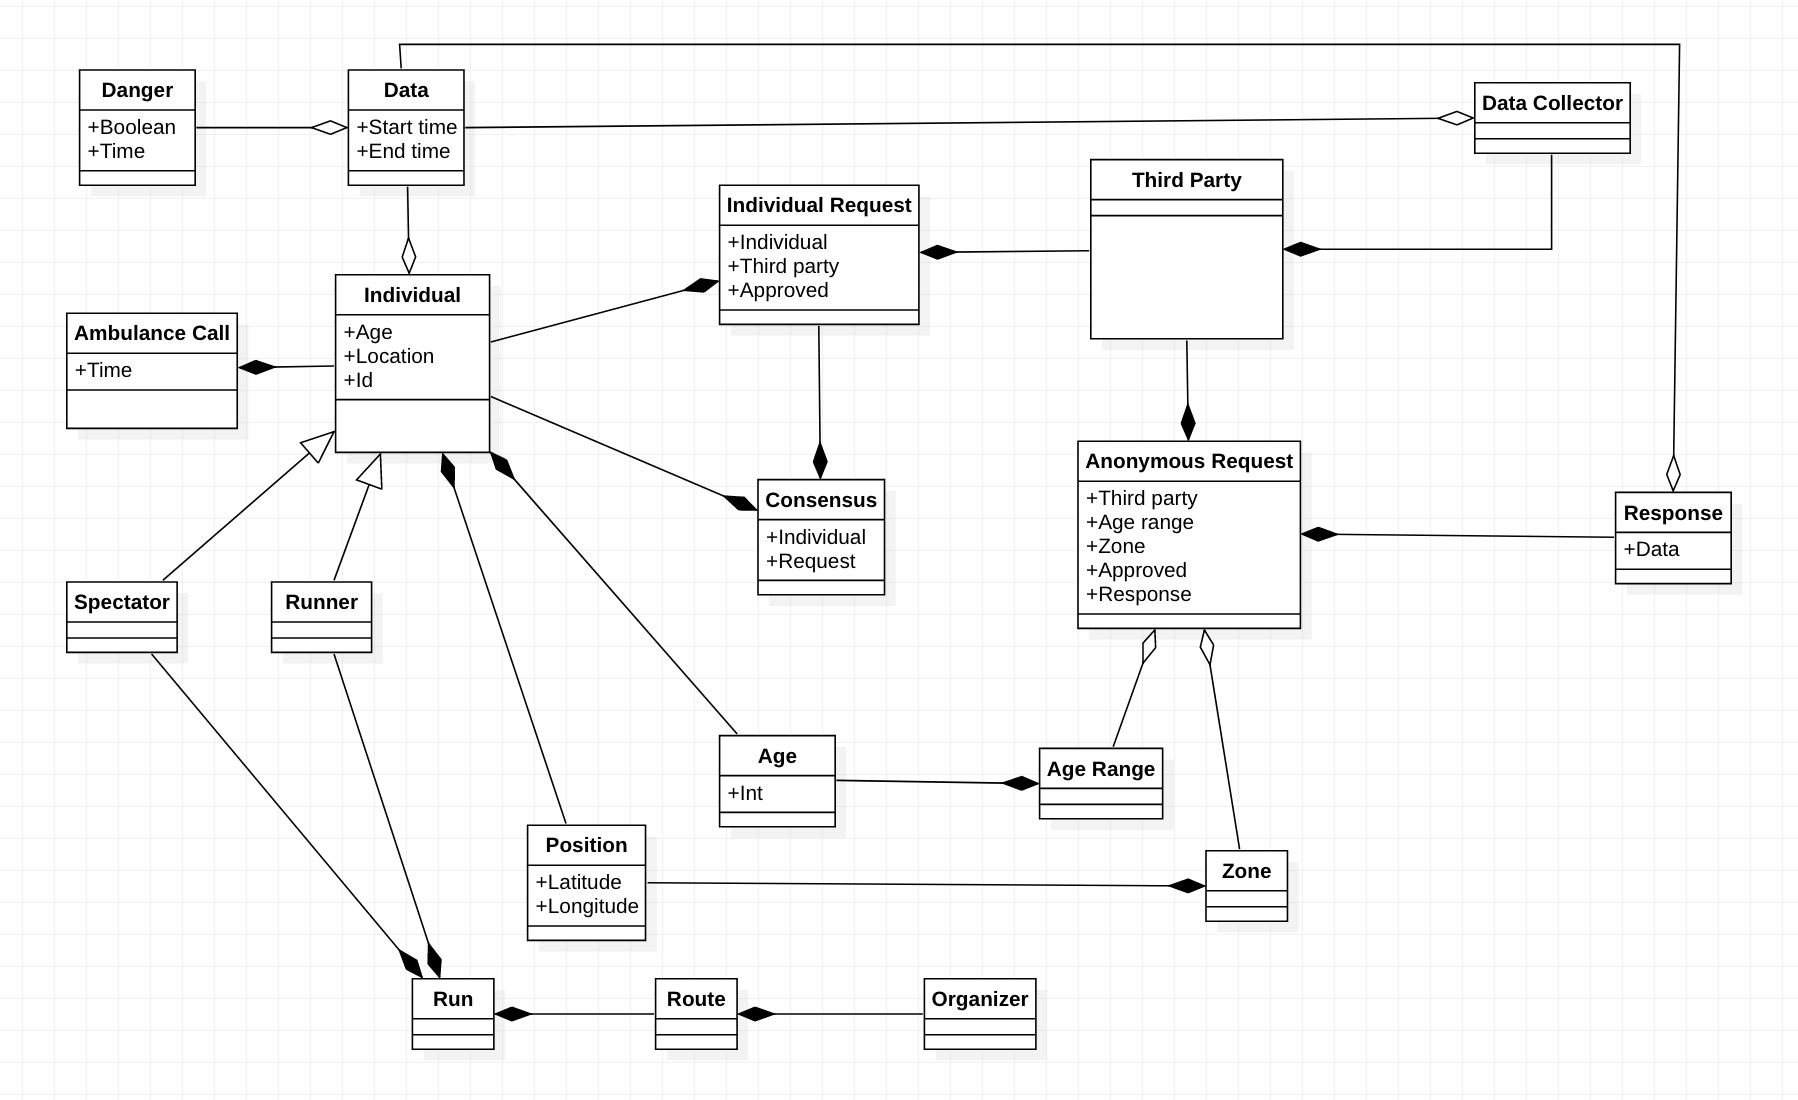
\includegraphics[width=\linewidth]{UML1-0.png}
	\end{figure}
	
	\end{legal}
\end{document}